\newpage
\subsection{Caso d'uso UC11: Visualizzazione pagina utente}
\label{UC11}
\begin{figure}[ht]
	\centering
	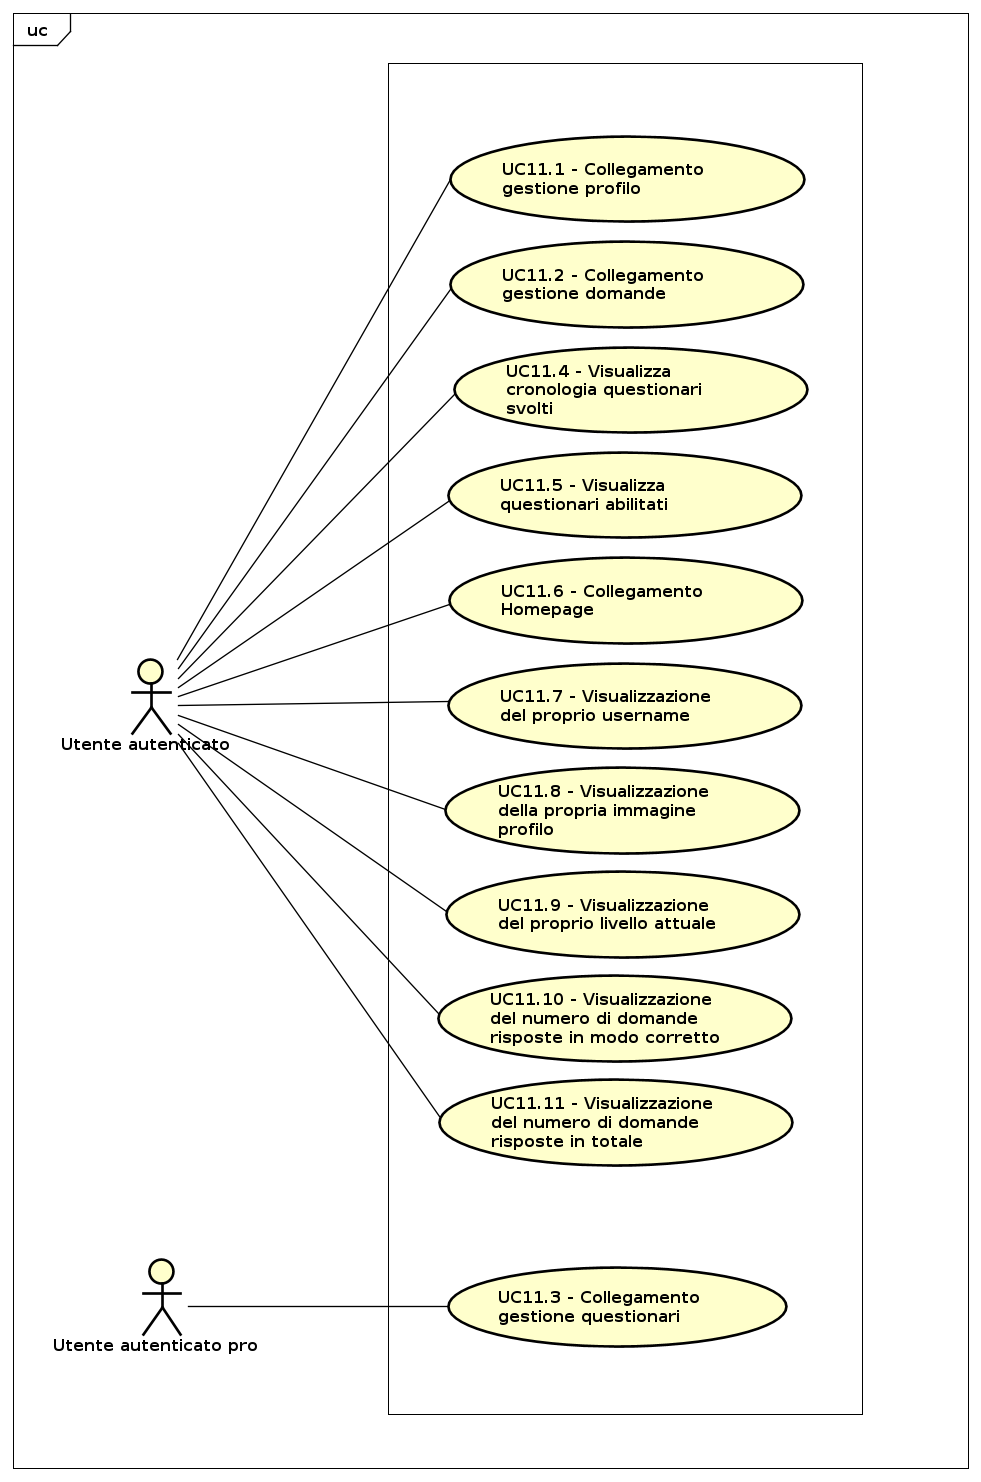
\includegraphics[scale=0.40]{UML/UC11.png}
	\caption{UC11: Gestione pagina utente}
\end{figure}
\FloatBarrier
\begin{itemize}
\item\textbf{Attori}: utente autenticato, utente autenticato pro;
\item\textbf{Descrizione}: da questa pagina l'attore può: 
\begin{itemize}
	\item Visualizzare tutti i dati del proprio profilo;
	\item Visualizzare tutti i dati sugli allenamenti;
	\item Visualizzare le statistiche dei questionari svolti;
	\item Visualizzare la cronologia dei questionari svolti;
	\item Accedere alla parte del sistema che permette di modificare il profilo;
	\item Accedere alla parte del sistema che permette di aggiungere nuove domande;
	\item Accedere alla parte del sistema che permette di creare questionari, se è un \uaupro{}.
\end{itemize}
\item\textbf{Precondizione}: il sistema mostra la pagina dell'utente;
\item\textbf{Postcondizione}: l'attore ha visualizzato i suoi dati come richiesto al sistema;
\item\textbf{Scenario principale}:
\begin{itemize}
\item L'attore può scegliere di andare alla pagina di gestione del profilo (UC11.1);
\item L'attore può scegliere di andare alla pagina di gestione delle domande (UC11.2);  
\item L'attore, solo l'\uaupro{} in questo caso, può scegliere di andare alla pagina di gestione dei questionari (UC11.3);
\item L'attore può scegliere di andare alla pagina di visualizzazione della cronologia dei questionari svolti (UC11.4);
\item L'attore può scegliere di andare alla pagina di visualizzazione dei questionari abilitati (UC11.5);
\item L'attore può scegliere di andare alla pagina principale (UC11.6);
\item L'attore visualizza il proprio username (UC11.7);
\item L'attore visualizza la propria immagine profilo (UC11.8);
\item L'attore visualizza il proprio livello attuale (UC11.9);
\item L'attore visualizza il numero di domande risposte in modo esatto (UC11.10);
\item L'attore visualizza il numero di domande risposte in totale (UC11.11).
\end{itemize}
\item\textbf{Inclusioni}: l'attore può compilare un questionario (UC7).
\end{itemize}

\subsubsection{Caso d'uso UC11.1: Collegamento gestione profilo}
\begin{itemize}
\item\textbf{Attori}: utente autenticato, utente autenticato pro;
\item\textbf{Descrizione}: l'attore viene portato nella pagina di gestione del profilo dove può modificare liberamente tutti i suoi dati;
\item\textbf{Precondizione}: il sistema mostra la pagina dell'utente;
\item\textbf{Postcondizione}: il sistema visualizza la pagina di gestione del profilo;
\item\textbf{Scenario principale}: l'attore si trova nella pagina di gestione del profilo e potrà attuare tutte le modifiche desiderate.
\end{itemize}

\subsubsection{Caso d'uso UC11.2: Collegamento gestione delle domande}
\begin{itemize}
\item\textbf{Attori}: utente autenticato, utente autenticato pro;
\item\textbf{Descrizione}: l'attore viene portato nella pagina di gestione delle domande dove può inserire o modificare le sue domande;
\item\textbf{Precondizione}: il sistema mostra la pagina dell'utente;

\item\textbf{Postcondizione}: il sistema visualizza la pagina di gestione delle domande;
\item\textbf{Scenario principale}: l'attore si trova nella pagina di gestione delle domande e potrà attuare tutte le modifiche desiderate.
\end{itemize}

\subsubsection{Caso d'uso UC11.3: Collegamento gestione questionari}
\begin{itemize}
\item\textbf{Attori}: utente autenticato pro;
\item\textbf{Descrizione}: l'attore viene portato nella pagina di gestione dei questionari dove può compiere tutte le azioni possibili sui questionari;
\item\textbf{Precondizione}:il sistema mostra la pagina dell'utente;
\item\textbf{Postcondizione}: il sistema visualizza la pagina di gestione dei questionari;
\item\textbf{Scenario principale}: l'attore si trova nella pagina di gestione dei questionari e potrà attuare tutte le modifiche desiderate.
\end{itemize}

\subsubsection{Caso d'uso UC11.4: Visualizzazione cronologia questionari svolti}
\label{UC11.4}
\begin{figure}[h]
	\centering
	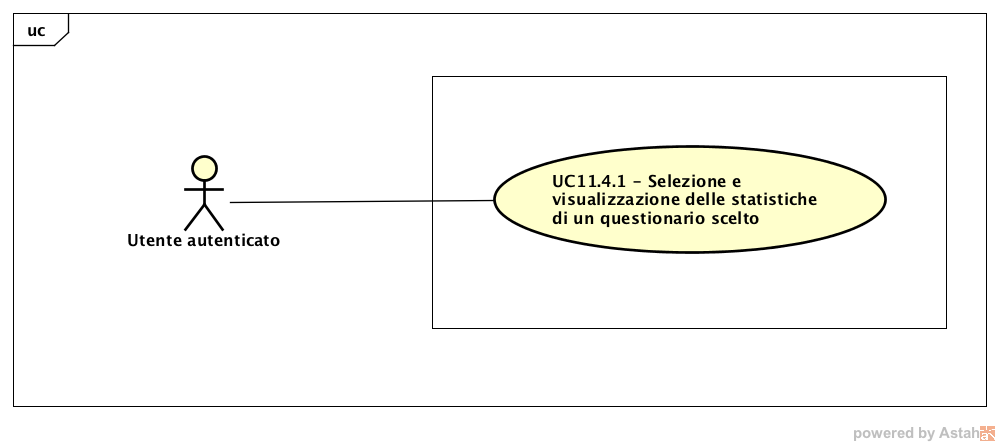
\includegraphics[scale=0.5]{UML/UC11_4.png}
	\caption{UC11.4: Visualizzazione cronologia questionari svolti}
\end{figure}
\begin{itemize}
\item\textbf{Attori}: utente autenticato, utente autenticato pro;
\item\textbf{Descrizione}: il sistema mostra la pagina dell'utente;
\item\textbf{Precondizione}: l'attore si trova nella propria pagina utente e ha compilato almeno un questionario;
\item\textbf{Postcondizione}: il sistema visualizza la cronologia dei questionari;
\item\textbf{Scenario principale}: l'attore può visualizzare le statistiche di un questionario (UC11.4.1).
\end{itemize}

\subsubsection{Caso d'uso UC11.4.1: Selezione e visualizzazione delle statistiche di un questionario scelto}
\begin{itemize}
\item\textbf{Attori}: utente autenticato, utente autenticato pro;
\item\textbf{Descrizione}: l'attore può selezionare un questionario fra quelli presenti nella cronologia e quindi visualizzarne le statistiche;
\item\textbf{Precondizione}: il sistema mostra all'attore tutti i questionari da lui svolti;
\item\textbf{Postcondizione}: il sistema ha mostrato all'attore le statistiche del questionario selezionato;
\item\textbf{Scenario principale}: l'attore si trova nella pagina dedicata alla visualizzazione delle statistiche di un particolare questionario da lui scelto.
\end{itemize}

\subsubsection{Caso d'uso UC11.5: Visualizzazione questionari abilitati}
\label{UC11.5}
\begin{figure}[h]
	\centering
	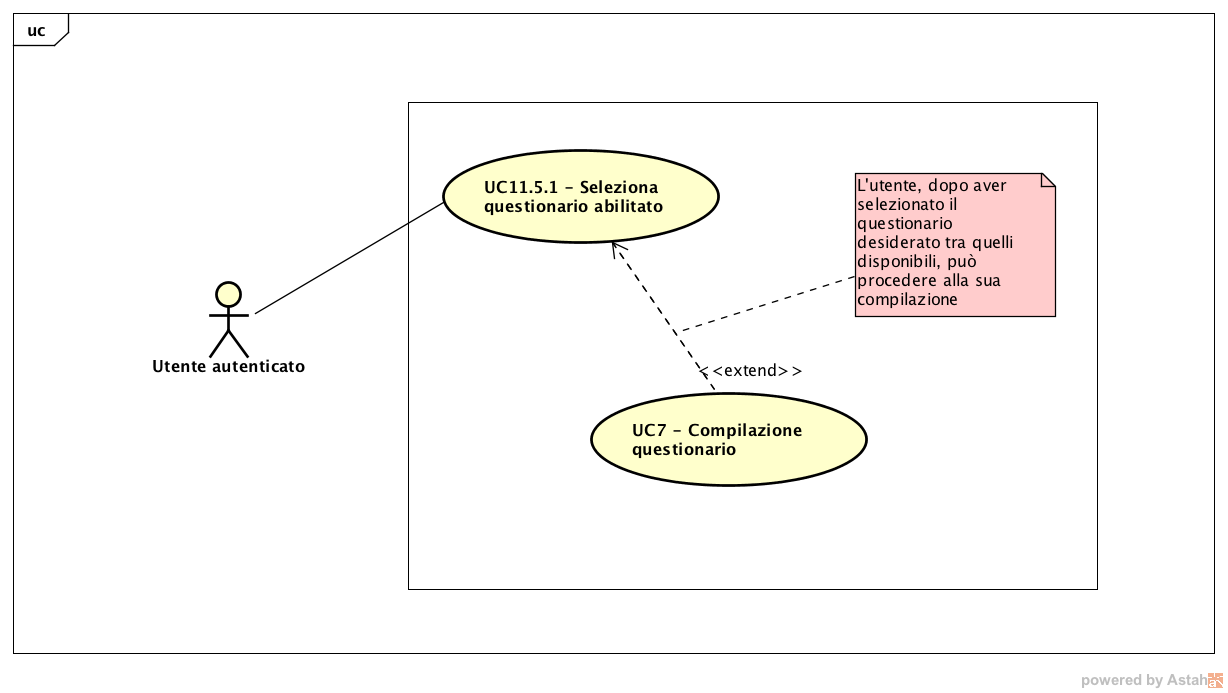
\includegraphics[scale=0.5]{UML/UC11_5.png}
	\caption{UC11.5: Visualizza questionari abilitati}
\end{figure}
\begin{itemize}
\item\textbf{Attori}: utente autenticato, utente autenticato pro;
\item\textbf{Descrizione}: l'attore può visualizzare la lista dei questionari a cui è stato abilitato da parte dell'utente autenticato pro proprietario del questionario.
\item\textbf{Precondizione}: il sistema mostra all'attore la propria pagina utente;
\item\textbf{Postcondizione}: il sistema ha mostrato all'attore tutti i questionari a cui è stato abilitato;
\item\textbf{Scenario principale}: l'attore può selezionare un questionario abilitato (UC11.5.1).
\end{itemize}

\subsubsection{Caso d'uso UC11.5.1: Seleziona questionario abilitato}
\begin{itemize}
\item\textbf{Attori}: utente autenticato, utente autenticato pro;
\item\textbf{Descrizione}: l'attore può selezionare un questionario a cui è stato abilitato e compilarlo;
\item\textbf{Precondizione}: il sistema mostra la pagina di tutti i questionari a cui l'utente è stato abilitato;
\item\textbf{Postcondizione}: l'attore ha selezionato un questionario a cui è stato abilitato;
\item\textbf{Scenario principale}: l'attore seleziona un questionario a cui è stato abilitato;
\item \textbf{Estensioni}: l'utente può compilare un questionario (UC7).
\end{itemize}

\subsubsection{Caso d'uso UC11.6: Collegamento Homepage}
\begin{itemize}
\item\textbf{Attori}: utente autenticato, utente autenticato pro;
\item\textbf{Descrizione}: l'attore può tornare alla pagina iniziale;
\item\textbf{Precondizione}: il sistema mostra la pagina dell'utente;
\item\textbf{Postcondizione}: il sistema visualizza la pagina iniziale;
\item\textbf{Scenario principale}: l'attore seleziona l'opzione per andare nella pagina iniziale.
\end{itemize}

\subsubsection{Caso d'uso UC11.7: Visualizzazione del proprio username}
\begin{itemize}
	\item\textbf{Attori}: utente autenticato, utente autenticato pro;
	\item\textbf{Descrizione}: l'attore visualizza il proprio username;
	\item\textbf{Precondizione}: il sistema visualizza la pagina utente;
	\item\textbf{Postcondizione}: il sistema visualizza l'username dell'utente;
	\item\textbf{Scenario principale}: l'attore visualizza il proprio nome utente;
\end{itemize}

\subsubsection{Caso d'uso UC11.8: Visualizzazione della propria immagine profilo }
\begin{itemize}
	\item\textbf{Attori}: utente autenticato, utente autenticato pro;
	\item\textbf{Descrizione}: l'attore visualizza la propria immagine profilo;
	\item\textbf{Precondizione}: il sistema visualizza la pagina utente;
	\item\textbf{Postcondizione}: il sistema visualizza l'immagine profilo dell'utente;
	\item\textbf{Scenario principale}: l'attore visualizza la propria immagine profilo;
\end{itemize}

\subsubsection{Caso d'uso UC11.9: Visualizzazione del proprio livello attuale }
\begin{itemize}
	\item\textbf{Attori}: utente autenticato, utente autenticato pro;
	\item\textbf{Descrizione}: l'attore visualizza il proprio livello attuale;
	\item\textbf{Precondizione}: il sistema visualizza la pagina utente;
	\item\textbf{Postcondizione}: il sistema visualizza il livello attuale dell'utente;
	\item\textbf{Scenario principale}: l'attore visualizza il proprio livello attuale.
\end{itemize}

\subsubsection{Caso d'uso UC11.10: Visualizzazione del numero di domande risposte in modo esatto}
\begin{itemize}
	\item\textbf{Attori}: utente autenticato, utente autenticato pro;
	\item\textbf{Descrizione}: l'attore visualizza il numero di domande risposte in modo corretto;
	\item\textbf{Precondizione}: il sistema visualizza la pagina utente;
	\item\textbf{Postcondizione}: il sistema visualizza il numero di domande risposte in modo esatto dall'utente;
	\item\textbf{Scenario principale}: l'attore visualizza il numero di domande risposte in modo corretto.
\end{itemize}

\subsubsection{Caso d'uso UC11.11: Visualizzazione del numero di domande risposte in totale}
\begin{itemize}
	\item\textbf{Attori}: utente autenticato, utente autenticato pro;
	\item\textbf{Descrizione}: l'attore visualizza il numero di domande risposte in totale;
	\item\textbf{Precondizione}: il sistema visualizza la pagina utente;
	\item\textbf{Postcondizione}: il sistema visualizza il numero di domande risposte in totale dall'utente;
	\item\textbf{Scenario principale}: l'attore visualizza il numero di domande risposte in totale.
\end{itemize}